\chapter{Evaluation}
\label{sec:evaluation}
\minitoc
\vspace*{1cm}

WRITE INTRO

% NEW SECTION
\section{Methodology}
\label{sec:dockerStack}
For the evaluation of our tool, we opted for convenience to use Docker ~\cite{docker_def}, which we also discussed in Chapter ~\ref{sec:background}. Docker is a software that can package your application, its dependencies, system tools, system libraries and settings in a single comprehensive virtual container. This is because Docker is lightweight, portable and can improve application development and deployment considerably.

As we already mentioned in Chapter ~\ref{sec:architecture}, \pname{} is limited to web applications written in PHP. The most popular and widely deployed language for Web applications is undoubtedly PHP, powering more than 80\% of the top ten million websites and contributing to almost 140,000 open-source projects on GitHub ~\cite{githubinfo}. For this reasons, we opted to evaluate our tool on web-apps developed in PHP.

The first web application we test our tool on is WordPress. The WordPress CMS (Content Management System) ~\cite{docker_def} is one of the most popular open-source web application for managing and publishing content on the web, with nearly half of the top 1 million sites on the internet using it. While it powers more than a third of the web, what is more important about it, for us, is that it is written in PHP and widely used for building a variety of websites, ranging from simple blog spots to professional web sites. 

We tested our tool on second web application, Drupal CMS ~\cite{drupal}. Drupal is a free and open-source content-management framework written in PHP and distributed under the GNU General Public License. It is used as a back-end framework for at least 2.1\% of all Web sites worldwide ranging from personal blogs to corporate, political, and government sites.

Using Docker, and more specifically its docker-compose functionality, we where able to achieved a multi-container deployment through a single docker-compose YAML file for the following services:

\begin{itemize}
	\item {\tt NGINX }: An open-source, high-performance HTTP server which handles all the HTTP request made by \pname{} and forwarded to our WordPress or Drupal web applications.{~\cite{nginx}}
	\item {\tt WordPress and Drupal }: Both open-source CMS web application. Since having access to the code, we began by examining the existing system in terms of injecting bugs and performing our instrumentation.
	\item {\tt MariaDB }: A popular open source relational databases which we used to store and manipulate the WordPress data~\cite{mariadb}.
\end{itemize}

The official images for the above services can be found for free at Docker Hub. An illustration of the above infrastructure in the case of WordPress, can be viewed at Figure ~\ref{fig:multi-container}. Files and instructions for replicating this process can be found at the fuzzer's repository. The respective docker-compose can be seen at Appendix ~\ref{sec:appendixb}.

\begin{figure}[ht]
 \centering
 \captionsetup{justification=centering}
 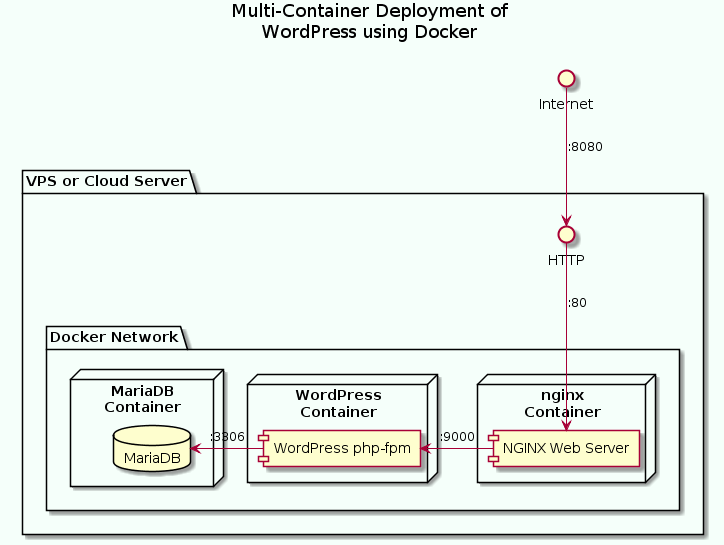
\includegraphics[width=\linewidth]{figures/multi-container.png}
 \caption{Evaluation followed the above Multi-Container Deployment of WordPress using Docker ~\cite{multi-container}.}
 \label{fig:multi-container}
\end{figure}

\section{Automated Vulnerability Addition}\label{sec:automated}
Evaluating fuzzing processes has proven to be a challenging task ~\cite{klees2018Evaluation}. Migrating known vulnerabilities to existing software, in order to test the capabilities of the fuzzer in finding bugs, can be a tedious process ~\cite{bug-reproduction}. Thus, for evaluating \pname{}, but also other fuzzers for web applications, an automated bug injection methodology, inspired by LAVA ~\cite{dolan2016lava} was used for automatically injecting bugs in web applications written in PHP. Injecting vulnerabilities in web code, again, is challenging, since important tools used for analysing native code and injecting vulnerabilities (e.g., taint-tracking and information-flow frameworks), are not available for web applications. To overcome this lack of available tools, the vulnerability injection methodology leverages the instrumentation infrastructure we use for building \pname{}, in the first place. The automated bug injection method is able to inject hundreds of common vulnerabilities such as Reflected Cross-Site Scripting in reasonable time. Details about the automated vulnerability addition, like the instrumentation, are out of the scopes of this thesis.

\section{Evaluation Details}
For the evaluation of \pname{}'s performance we used two Ubuntu 18.04 LTS Linux machines both possessing a quad-core Intel® Xeon® W-2104 Processor @3.20 GHz and 64GB of RAM. Targeted web applications consist of (a) an instrumented WordPress 5.5.1 with artificial bugs (b) a vanilla  WordPress 5.5.1 with artificial bugs, and (c) an instrumented Drupal 9.0.6. The term vanilla refers to web-apps in their original form, with no customizations or frameworks added to them. All artificial bugs where created with the automated vulnerability injection tool mentioned in  Section ~\ref{sec:automated}. Using this methodology, we managed to inject 150 identical Reflected Cross-Site Scripting bugs successfully in both the instrumented and vanilla versions of WordPress. Lastly, the Docker Stack of services described in Section ~\ref{sec:dockerStack} is deployed and running the aforementioned web applications.

For evaluating the performance of \pname{}, the following metrics are used:
\begin{itemize}
	\item {\tt Vulnerabilities Detected}: Number of Reflected Cross-Site Scripting bugs reported by \pname{}.
	\item {\tt Throughput}: Requests made per second.
	\item {\tt Global Code Coverage}: Accumulated coverage score of the web application's code.
\end{itemize}

To compare the Vulnerabilities Detected and the Throughput of \pname{} against other black-box fuzzers we use Wfuzz ~\cite{wfuzz}, Burp Suite Professional ~\cite{burp} and OWASP ZAP ~\cite{ owaspzap}. All three of this tools are consider essential in any penetration tester's arsenal as their included by default in Kali Linux and are widely used in Capture The Flag competitions such as DEF CON. Other tools; including \emph{nikto, skipfish and wapiti} where also used during the evaluation phase but as the were not able to uncover any real or artificially injected bugs we opted not to include them any further in our evaluation. The main comparison was made against Wfuzz due to its ease of operation and ease to extend. The choice of Wfuzz as the main comparison of our tool is further elaborated in Chapter ~\ref{sec:discussion}.

\section{Vulnerabilities Detected}
To evaluate how well \pname{} performs in terms of bug detection, we injected 150 artificial  Reflected Cross-site bugs, with the methodology we discussed in Section ~\ref{sec:automated} and 4 real Reflected Cross-site Scripting bugs to the instrumented version of WordPress, and tested how 3 well-known black-box fuzzers perform in comparison to \pname{}. The real-life RXSS bugs were found from CVE ~\cite{cve} and have the following ids: CVE-2018-7280, CVE-2019-11843, CVE-2020-7104, CVE-2020-7107.

\begin{table}[ht]
\centering
 \begin{tabular}{@{}|l|l|l|l|l|@{}}
 \hline
  \multicolumn{5}{|c|}{\textit{\textbf{Vulnerability Detection}}} \\
 \hline
 \textbf{Tool} & \textbf{Version} & \textbf{Real Bugs} & \textbf{Artificial Bugs} & \textbf{Runtime} \\ 
 \hline\hline
 \pname{} & 1.0.0 & 1 & 30 & 65h  \\ 
 \hline
 Wfuzz & 2.4.5 & 1 & 28 & 65h  \\ 
 \hline
 Burp Suite Professional & 2020.9.2 & 1 & 0 & 7h \\ 
 \hline
 OWASP ZAP  & 2.9.0 & 1 & 0 & 1h  \\
 \hline
 \end{tabular}
 \caption{Summary of the vulnerability detection evaluation that includes the findings of \emph{4} fuzzers including \pname{}. The WordPress web-app included \emph{4} RXSS bugs found from CVE {~\cite{cve}} and \emph{150} artificial RXSS bugs injected manually.}

 \label{tools_table}
\end{table}

When analysing the specifics of the 4 real-life RXSS vulnerabilities that where manually injected, it was realised that 1 out of these depends on JavaScript code to create its triggering link dynamically in the form of an anchor element. The other 3 depend on JavaScript code to dynamically append the vulnerable POST parameter upon form submission. Also, for the vulnerability CVE-2018-7280 to be triggered it is compulsory that the XSS payload be injected inside a specific JSON object at one of the vulnerable form's parameters. As Table ~\ref{tools_table}, all tools involved in the evaluation only managed to find one real-life RXSS bug. This is because none of them employ complex enough JavaScript code analysis nor do they run a request's client side code so as to uncover these dynamic links and parameters.

At this point, it is important to note that vulnerability scanners such as Burp Suite Professional provide a Proxy service that can intercept web browsing traffic so that requests created dynamically by client side code can be fuzzed as well. Nevertheless, we opted to avoid this kind of features since \pname{} currently lacks this functionality and thus, it would be an unfair comparison.

As we can clearly observe from Table ~\ref{tools_table}, results of all fuzzers for real-life bugs are disappointing. For this reason, we further evaluated the fuzzing tools on how well they perform with artificially injected bugs (Section ~\ref{sec:automated}). Because OWASP ZAP and Burp Suite Professional do not generate the required format of injection payloads unless advanced features and modifications are in place, they were unable to detect any of the artificially injected bugs. Using their advanced features requires extensive research and training as the learning curve is steep, hence we opted to customise Wfuzz only since it is more straight forward.

To make fair comparison of the vulnerability detecting capabilities of \pname{} and Wfuzz, some modification have been made to the latter since originally the tool was meant to be a brute forcer and not a black-box fuzzer. Firstly, an independent crawling process was added at the start to dynamically infer the control flow of the web application. The findings are stored and fed to Wfuzz as a list of fuzz targets. Utilising the Python module version of Wfuzz, a Python script was created that fuzzes the list of links found by the crawler indefinitely. Payloads used during the fuzzing process are customised to resemble the mutated payloads that \pname{} uses. They consist of random strings, HTML syntax tokens, and random numbers all concatenated with the same XSS payloads that webFuzz uses from its corpus described in Chapter ~\ref{sec:architecture}.

\begin{figure}[!htb]
  \centering 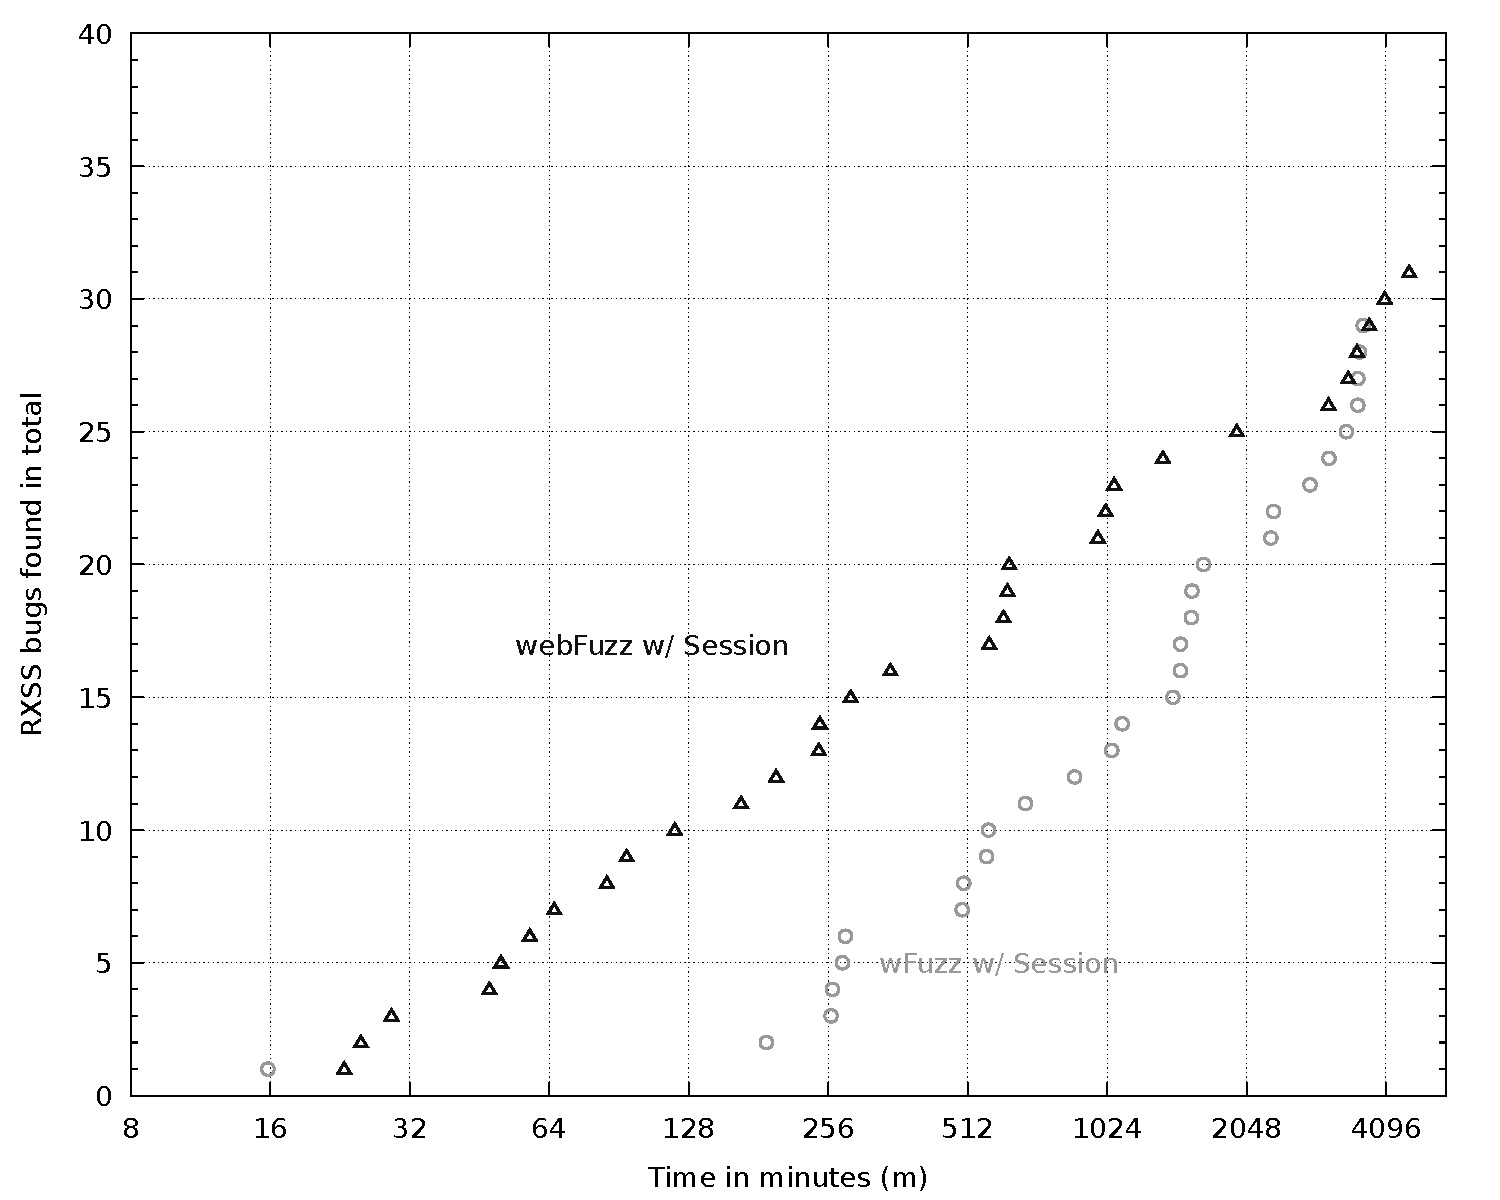
\includegraphics[width=\linewidth]{figures/plot_bugs.pdf}
  \caption{ Artificial Reflected Cross-Site Scripting bugs detected over time by \pname{} and Wfuzz. \pname{} manages to uncover more bugs more quickly during the fuzzing process.} 
  \label{fig:plot_rxss}
\end{figure}

The results of our 65-hour long experiment, comparing Wfuzz and \pname{} in terms of artificial RXSS bugs found can be seen at Figure ~\ref{fig:plot_rxss}. Although \pname{} has the lead through the entire experiment, the difference kept on decreasing until towards the end where the difference is marginal. By taking advantage of the instrumentation feedback-loop, \pname{} could detect the artificial bugs faster than Wfuzz's brute force approach. Whenever a digit of a magic
number, situated in a vulnerable payload, is guessed correctly our fuzzing tool will detect this change and will thus prioritize the request that causes it. Using this method, the finding of a magic number is done in an incremental fashion - one correct digit at a time - which is much faster than guessing the whole number at once like Wfuzz does. As a real world analogy, each digit of the magic number can represent one correct mutation that gets us closer to the vulnerable basic block. A reason for the gradual decrease of webFuzz's detection performance lies in its growing request queue size. WordPress is composed out of approximately half a million Lines of Code(LoC), with 48,040 basic blocks instrumented in total.

\section{Throughput}
One reason for the effectiveness of fuzzers in uncovering vulnerabilities is their capability to test vast amounts of inputs per second. Thus, it is essential that the overhead caused by instrumentation does not degrade severely the web application's response time and that the fuzzer's processing time for each request is kept as brief as possible.

\begin{figure}[!htb]
  \centering 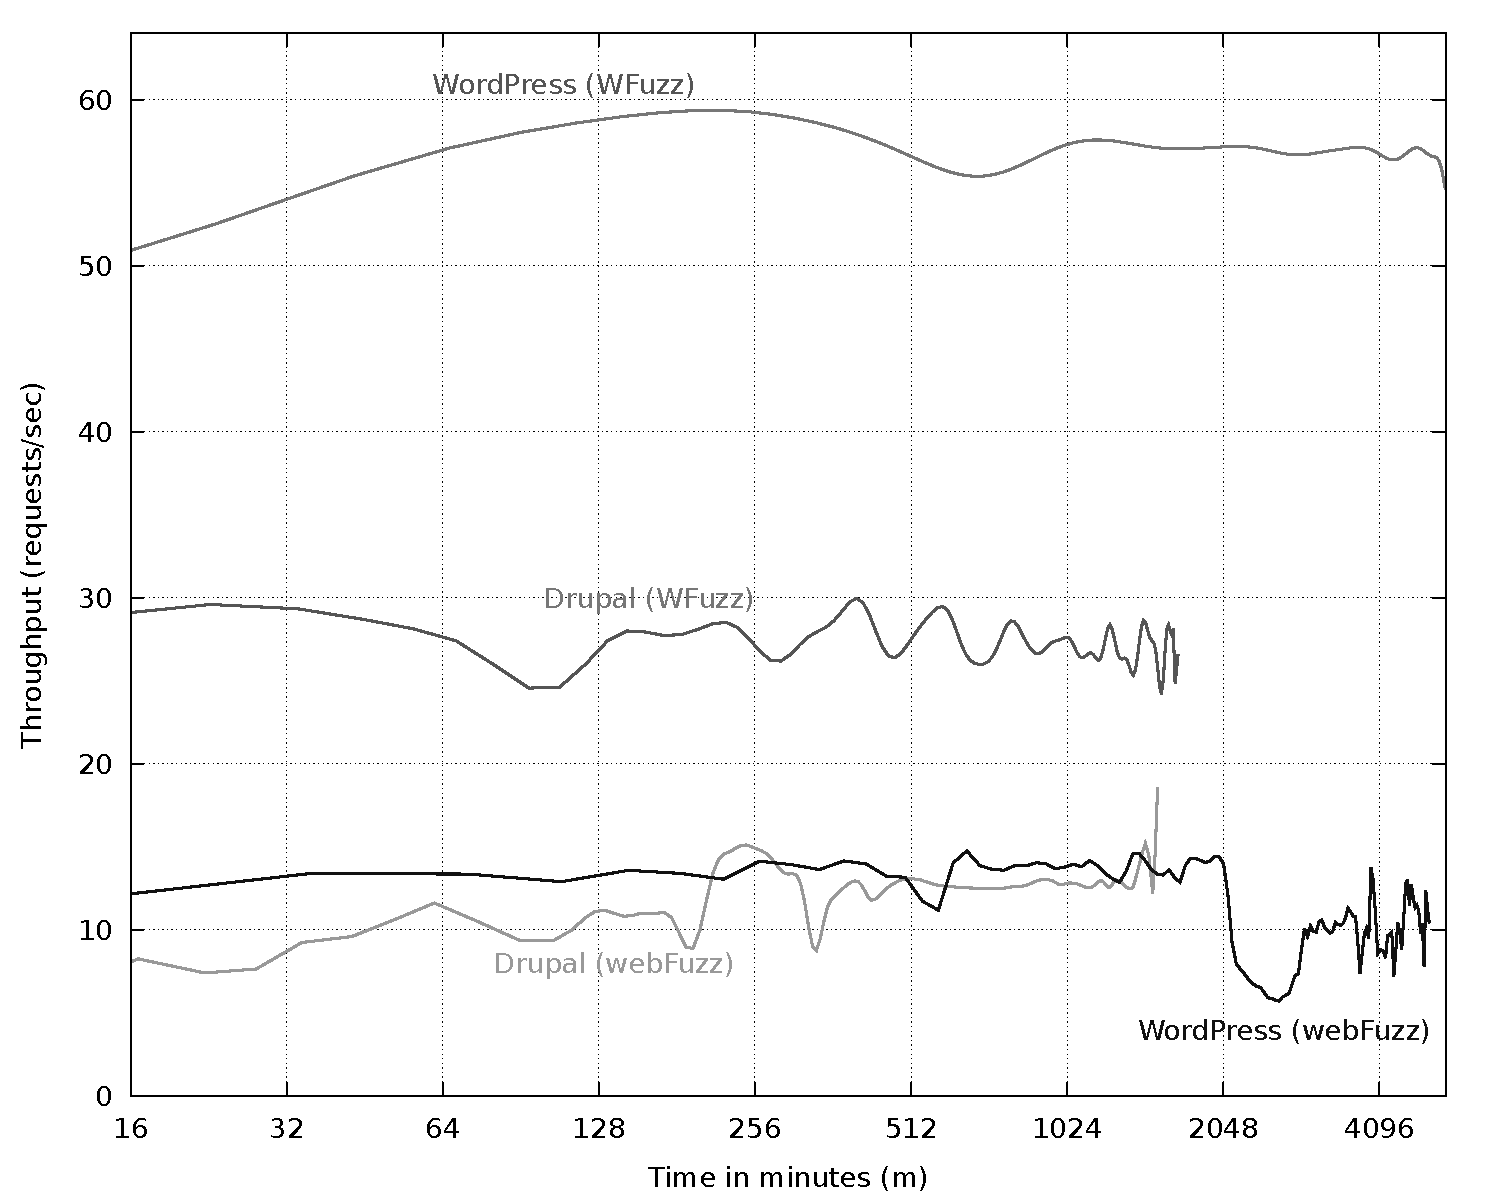
\includegraphics[width=\linewidth]{figures/plot_throughput.pdf}
  \caption{Requests made per second over time for three different scenarios. Both \pname{} and Wfuzz are evaluated on Drupal and WordPress. Wfuzz takes the lead with a difference.} 
  \label{fig:plot_throughput}
\end{figure}

As observed in Figure ~\ref{fig:plot_throughput}, the black-box version of Wfuzz has about \emph{3} times higher throughput than \pname{} in the case of Drupal and \emph{4.5} times in WordPress. This is plausible as the overhead added from instrumentation roughly doubles the page response time in the case of WordPress, and due to webFuzz's increased statefulness in tracking, analysing and ranking all the requests, increases the per request processing time.

After 2,048 minutes in WordPress using \pname{}, with an authenticated session established, the throughput is seen to plummet for a lengthy period of time. This implies that the fuzzer got stuck on fuzzing particular links that have lofty response times. The fact that the fuzzer keeps on fuzing these links means that they have have a high coverage score and mutating them is effective enough to trigger new code paths in them.

Looking at Figure ~\ref{fig:plot_throughput}, we can state with confidence that much has to be done to improve the throughput of \pname{}, since currently it is nowhere near that of native applications fuzzers such as AFL and EFS nor is it very comparable to black-box web fuzzers such as Wfuzz. Improvements are discussed in Chapter ~\ref{sec:discussion}.

\section{Global Code Coverage}
Utilizing the instrumentation feedback, \pname{} has calculated the Global Code Coverage for both authenticated and guest sessions of WordPress and for an authenticated session run of Drupal. Observing Figure ~\ref{fig:plot_coverage}, we can view how the aforementioned metric rises over time for the two authenticated session scenarios.

\begin{figure}[!htb]
  \centering 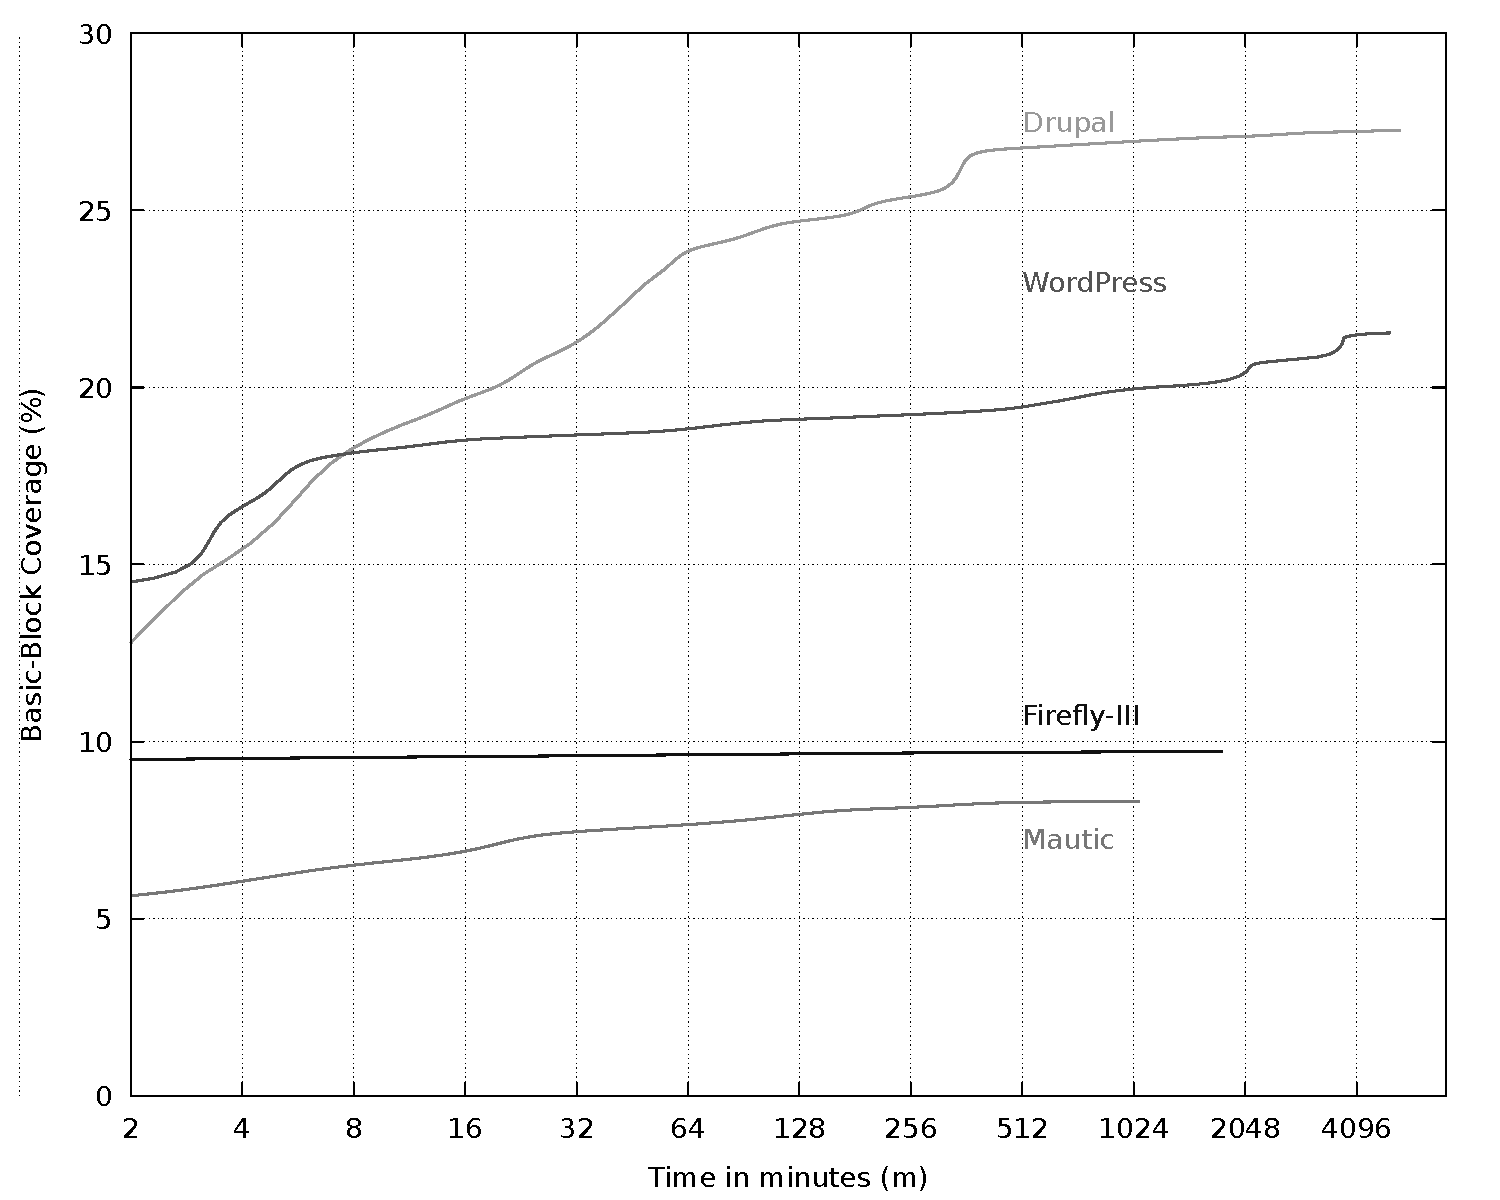
\includegraphics[width=\linewidth]{figures/plot_coverage.pdf}
  \caption{Three different execution scenarios and the accumulated code coverage gained over time in each one. Exponential increases witnessed at the start of the experiments are due to the initial exploration of the target web application's site map by the crawler.} 
  \label{fig:plot_coverage}
\end{figure}

During the not authenticated session scenario of WordPress, access is forbidden to various links such as Administrative Dashboard related links. For this reason, the code coverage calculated is the smallest and remains stagnant at about \emph{7\%} for the best part of the experiment. However, the authenticated sessions have access to the Administrative Dashboard provided by Drupal and WordPress, and have thus managed to achieve global code coverages as high as \emph{30\%} and \emph{21.5\%} respectively. 

An important thing to note here is that the code coverage achieved by \pname{} in the authenticated session run of WordPress indicates rises in the global code coverage even after 50 hours of execution time. A good signal that the mutation functions used are effective enough to trigger new code paths, even after the crawling process has finished.
 
\begin{figure}[!htb]
  \centering 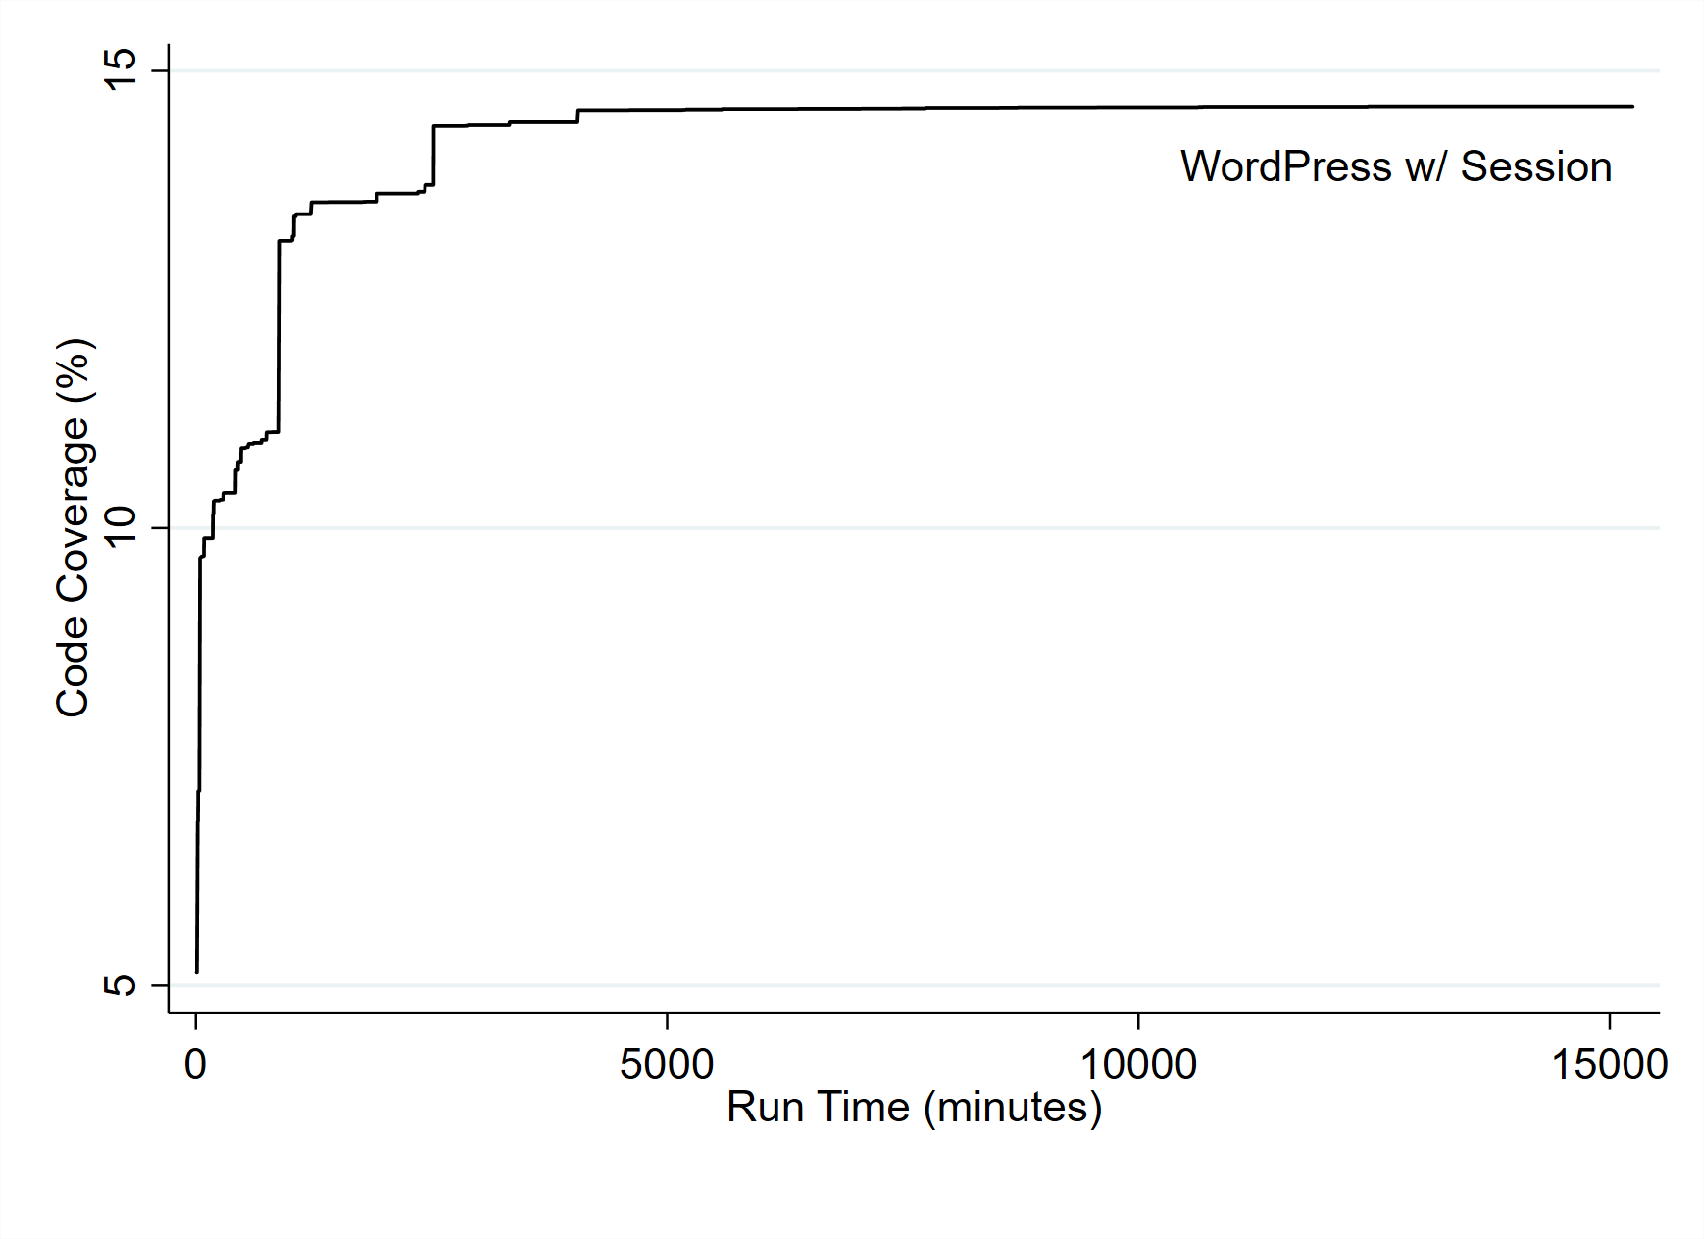
\includegraphics[width=\linewidth]{figures/plot_coverage2.pdf}
  \caption{Code coverage achieved by Wfuzz over time when fuzzing WordPress using an authenticated session. After running for approximately \emph{5000} minutes (3.5 days) the code coverage remained stagnant at \emph{14.6\%} for the rest of the experiment.}
  \label{fig:plot_coverage2}
\end{figure}

In Figure ~\ref{fig:plot_coverage2} we can see the Global Code Coverage achieved by a black-box fuzzer, Wfuzz, when fuzzing WordPress using an authenticated session. The peak of this experiment was reached in roughly \emph{3.5} days (5000 minutes) when code coverage of \emph{14.613\%} was reached. This experiment was done solely to check how well a black-box fuzzer performs in terms of code coverage against a gray-box fuzzer, like \pname{}, that leverages instrumentation feedback. When looking at both Figures ~\ref{fig:plot_coverage} and ~\ref{fig:plot_coverage2} we can state with confidence that the instrumentation feedback provides \pname{} the edge needed to surpass the performance of Wfuzz. More precisely, when both where fuzzing WordPress with an authenticated session, \pname{} managed to get almost \emph{1.5} times higher code coverage than Wfuzz. Wfuzz was left running for much longer time than \pname{} but with no luck since it stayed stagnant on the score it achieved in 3.5 days at \emph{14.613\%}.